\subsection{Home Assistant}

Bei Home Assistant handelt es sich um Open Source Software im Bereich Smart Home. Es zielt darauf
ab, die Privatsphäre der Nutzenden zu erhöhen, indem so weit wie möglich auf externe Server
verzichtet wird. Typischerweise wird Home Assistant auf einem Raspberry Pi betrieben, der sich in
der gleichen Wohneinheit \todo{Haus / Wohnung?} mit den zu kontrollierenden Geräten befindet.
\parencite{homeassistantHomeAssistant}

Im Folgenden werden die wichtigsten Konzepte für das Verständnis von Home Assistant vorgestellt.
\textbf{Integrationen} stellen Software dar, welche mit anderen Plattformen kommuniziert, und es
somit ermöglicht, Geräte von verschiedenen Herstellern einzubinden. Daraufhin sind diese als
\textbf{Geräte} in Home Assistant vertreten und stellen sogenannte \textbf{Entitäten} bereit, welche
den Zustand des Geräts beschreiben und kontrollieren. Auf Basis von Sensoren und Kontroll-Entitäten
können nun \textbf{Automatisierungen} erstellt werden. Diese bestehen aus \textbf{Auslösern}, welche
die Automatisierung starten und etwas beschreiben, was im Haus\todo{?} passiert (Beispiel: "Person
betritt Wohnzimmer."). Des Weiteren können \textbf{Bedingungen} angegeben werden, die zusätzliche
Tests darstellen, welche die Ausführung der Automatisierung verhindern können (Beispiel:
"Umgebungslicht ist unter 20 Lux."). Sobald die Automatisierung ausgelöst wurde und die Bedingungen
übereinstimmen, werden \textbf{Aktionen} ausgeführt. Diese steuern Geräte oder Entitäten und werden
standardmäßig als Liste ausgeführt (Beispiel: "Leselampe anschalten, Musik abspielen.").
\textbf{Skripte} sind Sammlungen von Aktionen, welche als eine Aktion wiederverwendet werden können.
\parencite{homeassistantConceptsTerminology} Sowohl Automatisierungen als auch Skripte werden als
\acs{YAML}-Dateien\footnote{\acs{YAML}: \acl{YAML}} gespeichert und können über einen visuellen
Editor bearbeitet werden. Dieser wird im Folgenden betrachtet.

\subsubsection{Editor zum Erstellen von Automatisierungen}
\begin{figure}[!ht]
  \minipage[t]{.49\textwidth}
  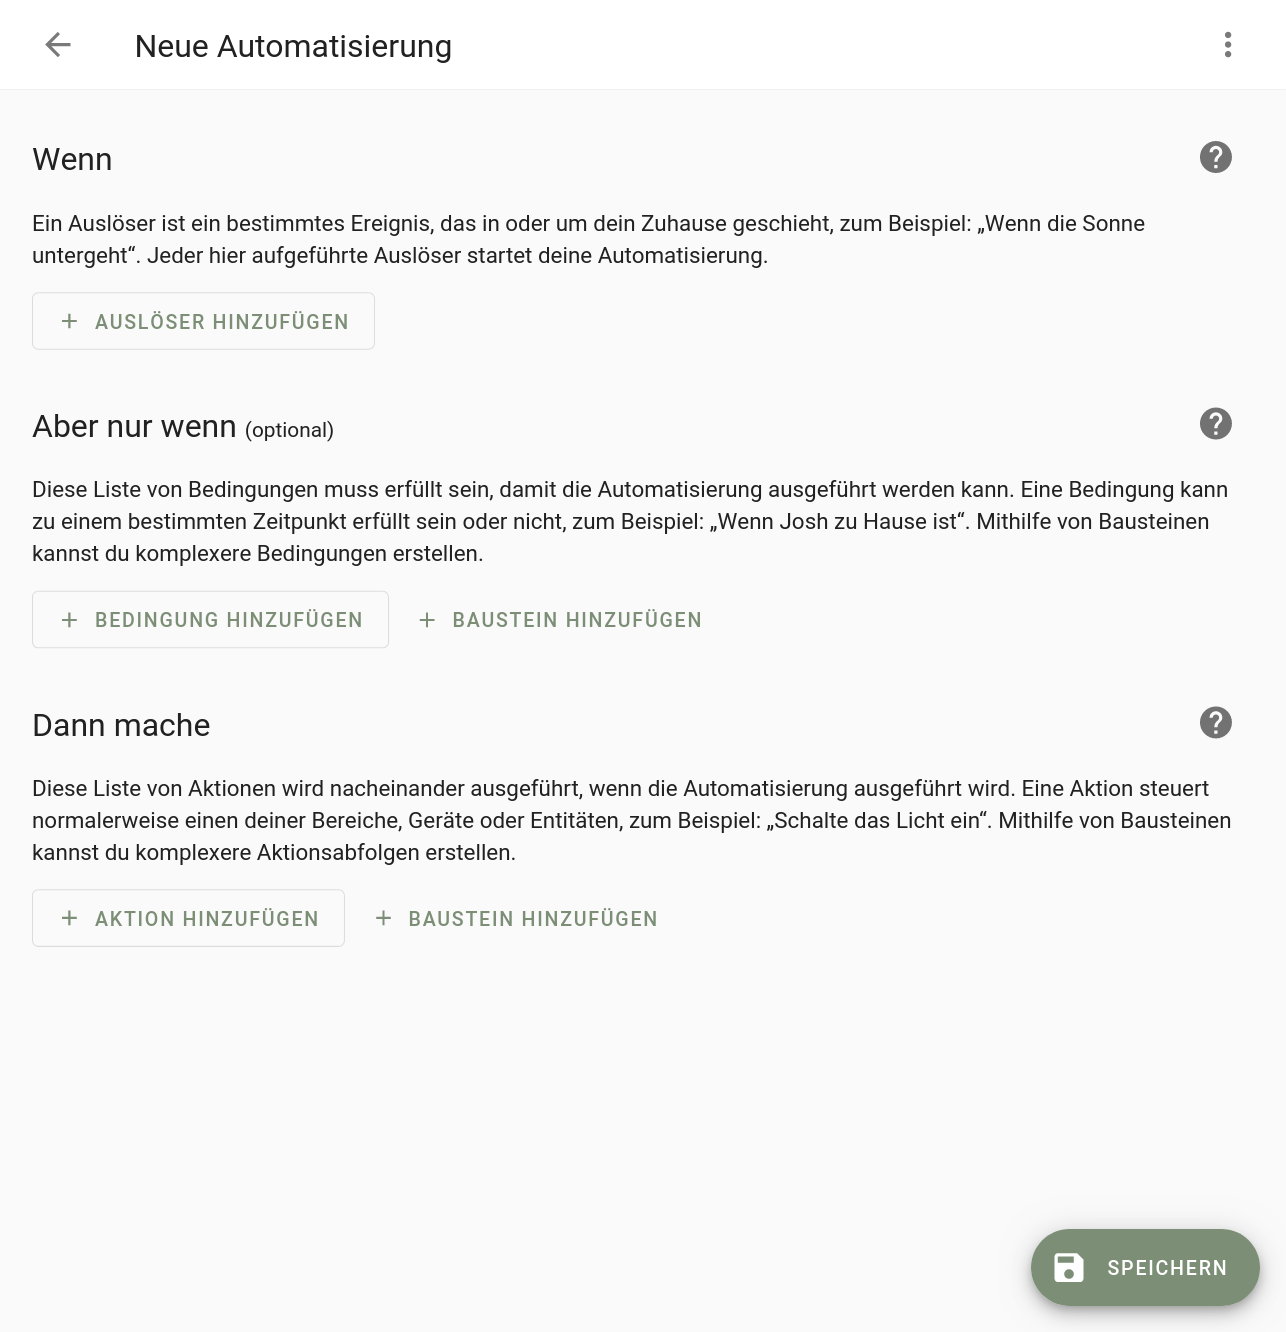
\includegraphics[width=\linewidth]{assets/hassio-automation-empty.png}
  \caption{Startpunkt der Erstellung einer Automatisierung in Home Assistant}
  \label{figure:hassio-automation-empty}
  \endminipage
  \hfill
  \minipage[t]{.49\textwidth}
  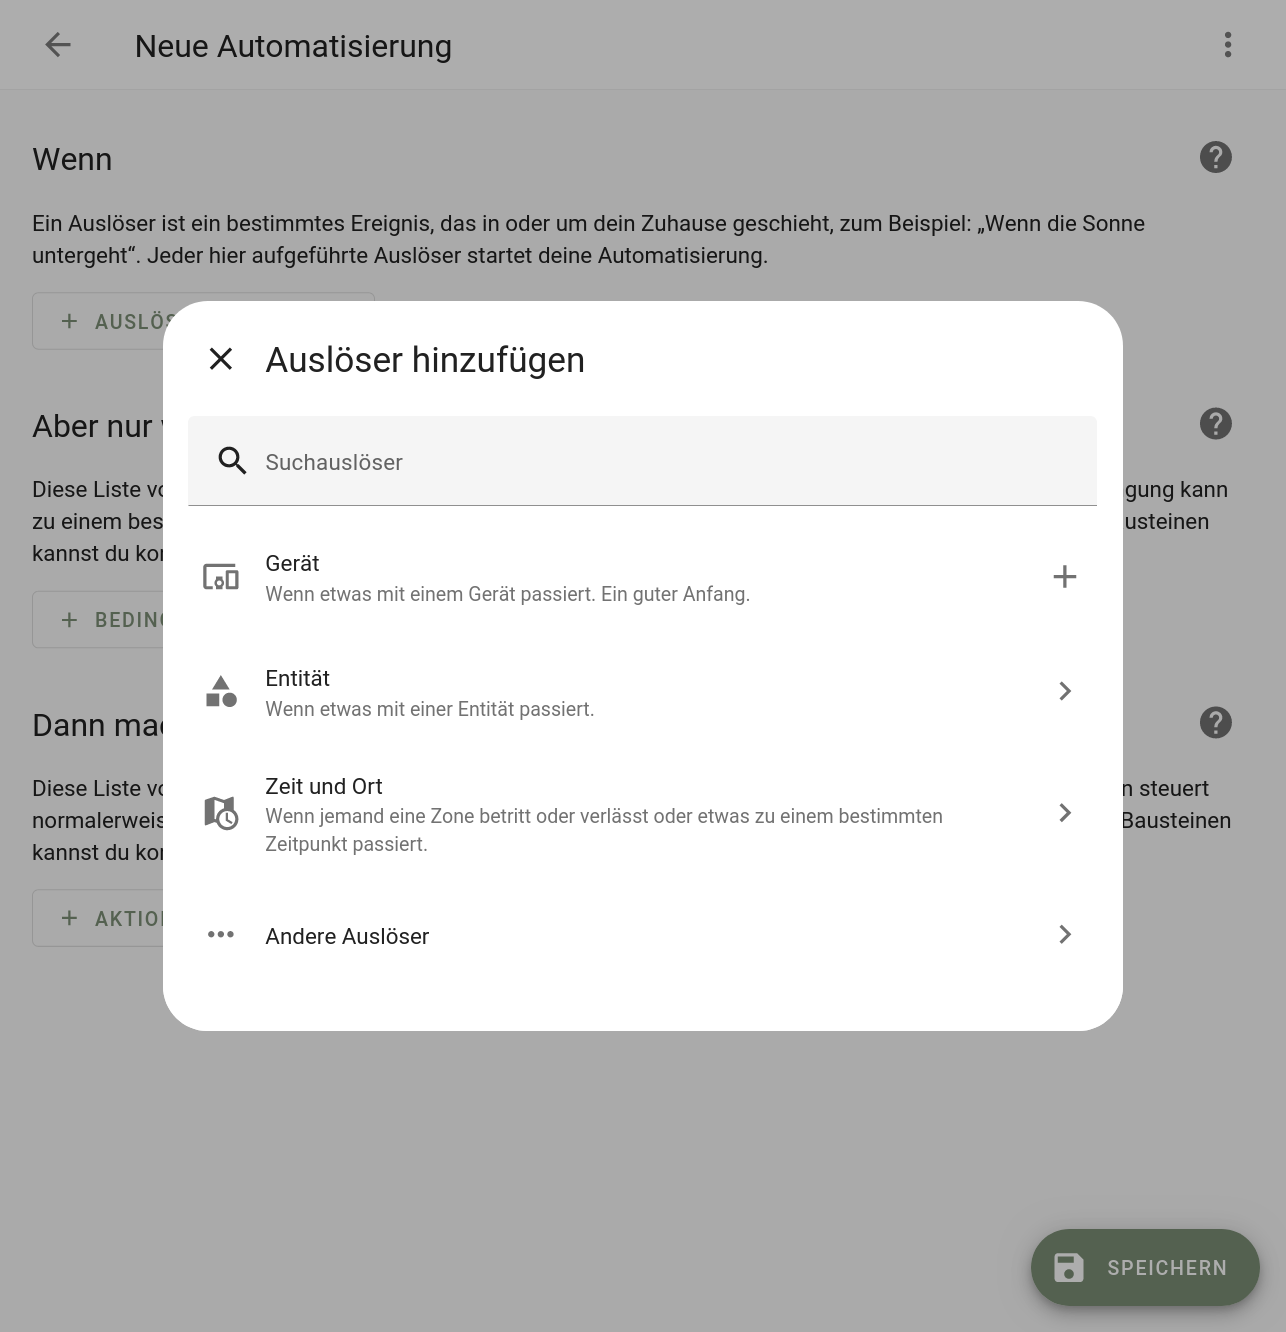
\includegraphics[width=\linewidth]{assets/hassio-automation-trigger-select-1.png}
  \caption{Auswahl eines Auslösers (1)}
  \label{figure:hassio-automation-trigger-select-1}
  \endminipage
\end{figure}

Abbildung \ref{figure:hassio-automation-empty} zeigt den Initialzustand bei der Erstellung einer
neuen Automatisierung. Die Ansicht ist in drei Abschnitte unterteilt, in der die drei relevanten
Bausteine angegeben werden können. Abschnitte, die noch keinen Baustein enthalten, verfügen über
einen Button zum Hinzufügen dieser. Der Button öffnet ein kontextabhängiges Pop-up-Fenster, wie in
Abbildung \ref{figure:hassio-automation-trigger-select-1} und
\ref{figure:hassio-automation-trigger-select-2} zu sehen. Je nach Typ des Bausteins werden dort
unterschiedliche Elemente angezeigt. So werden im Auswahlmenü für Auslöser (Abbildung
\ref{figure:hassio-automation-trigger-select-1}) nur passende Elemente gezeigt. In diesem Falle
können Auslöser die Zustände von Geräten oder Entitäten, sowie zeitliche und örtlich bedingte
Zustände sein. Sobald ein Auslöser ausgewählt wurde, können Einstellungen mit passenden UI-Elementen
bearbeitet werden. Diese Einstellungen sind spezifisch für die Art des ausgewählten Auslösers. In
Abbildung \ref{figure:hassio-automation-trigger} wurde der Auslöser "Zone" ausgewählt. Die Auswahl
der gemeinten Person und Zone erfolgt über Dropdowns, während die Angabe, ob es auf das Betreten
oder Verlassen der Zone geachtet werden soll, über einen Radiobutton gelöst wird. \todo{wo wird das
festgelegt? configuration schema?} Die verfügbaren Auslöser werden von Integrationen bereitgestellt
und per Programmcode mittels Python definiert \parencite{homeassistantDeviceAutomations2023}. In
anderen Teilen des Home Assistant Projektes werden die passenden \ac{UI}-Elemente per TypeScript
definiert \parencite{homeassistantHomeassistantFrontend}.

\begin{figure}[!ht]
  \minipage[t]{.49\textwidth}
  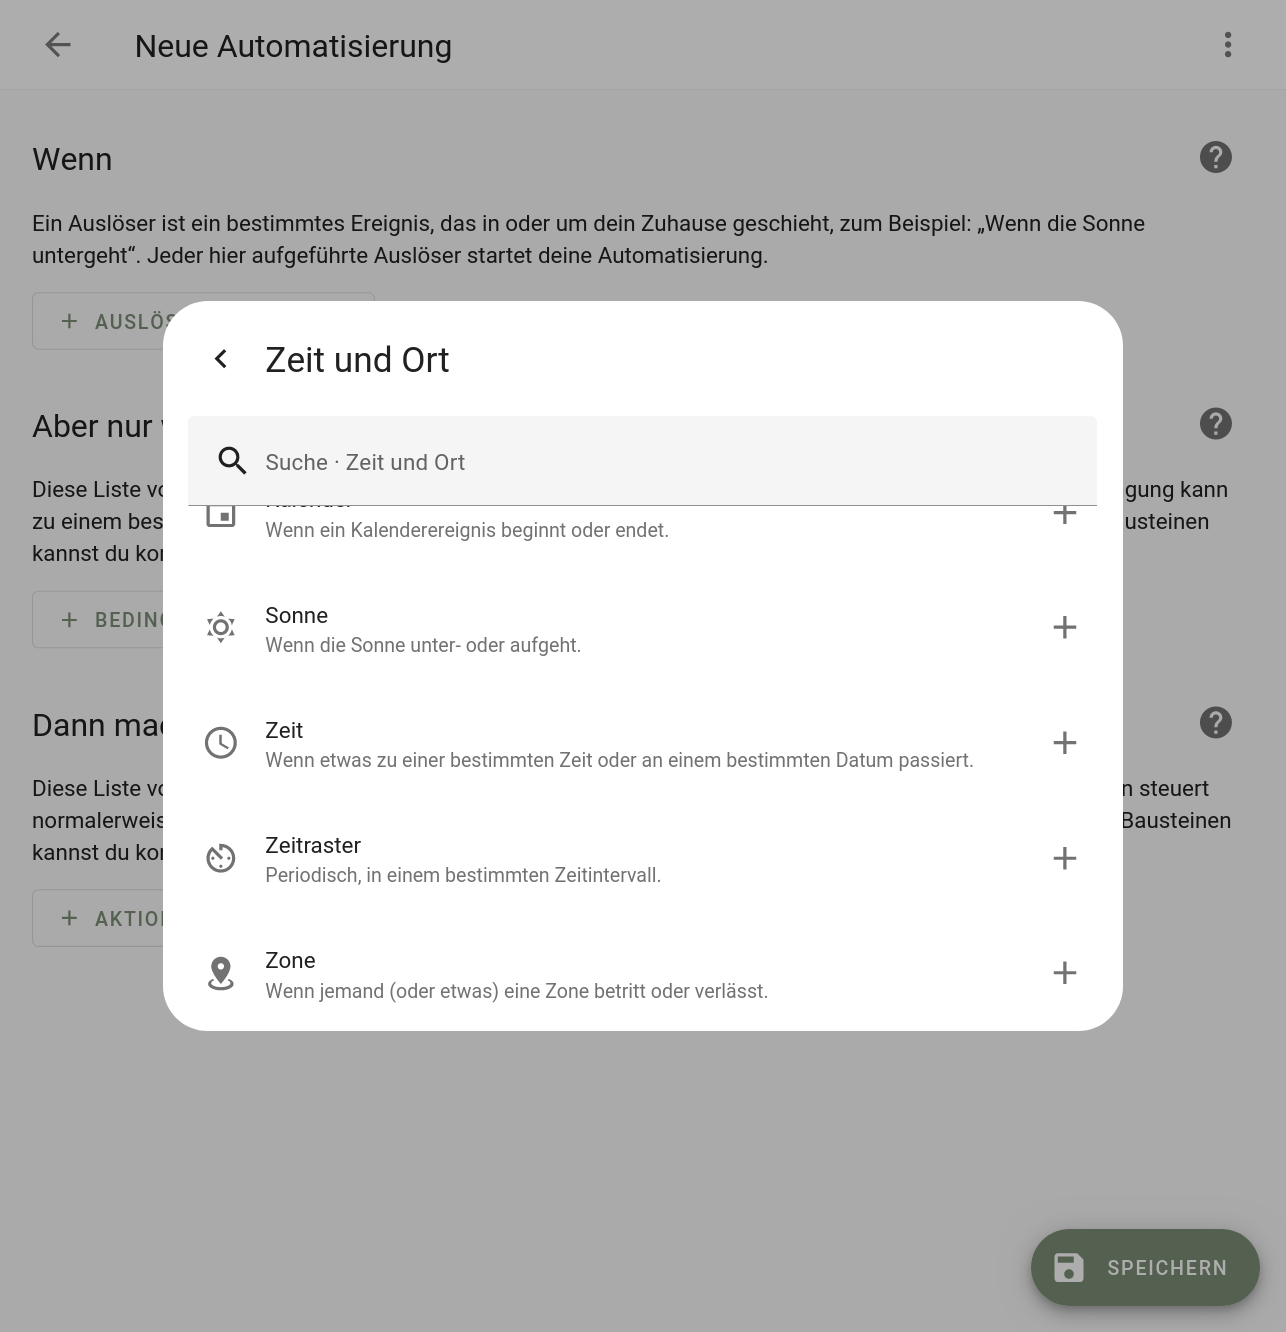
\includegraphics[width=\linewidth]{assets/hassio-automation-trigger-select-2.png}
  \caption{Auswahl eines Auslösers (2)}
  \label{figure:hassio-automation-trigger-select-2}
  \endminipage
  \hfill
  \minipage[t]{.49\textwidth}
  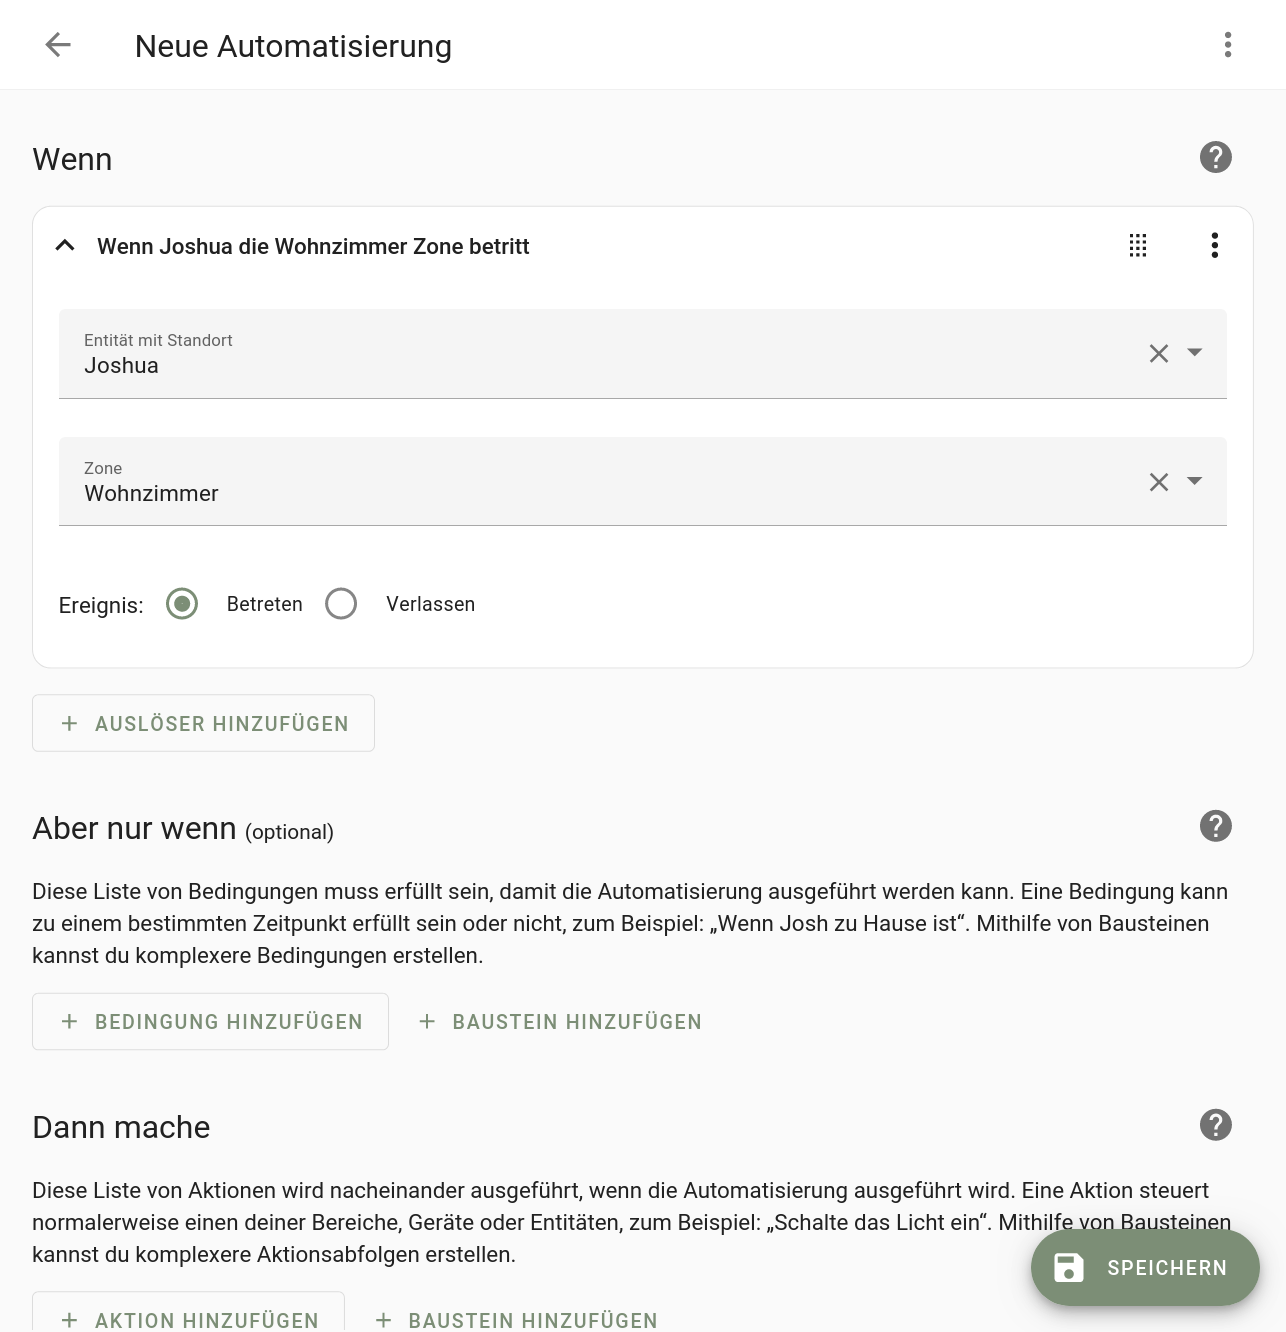
\includegraphics[width=\linewidth]{assets/hassio-automation-trigger.png}
  \caption{Angabe eines Auslösers in Home Assistant}
  \label{figure:hassio-automation-trigger}
  \endminipage
\end{figure}

Abbildung \ref{figure:hassio-automation-condition} zeigt eine angegebene Bedingung. In diesem Fall
wurde  die Bedingung "Numerischer Wert" mit der Entität "Umgebungslicht" ausgewählt und im Feld
"Unter" wurde der Wert 20 eingetragen. Dies hat den Effekt, dass die Automatisierung nur ausgeführt
wird, wenn das Umgebungslicht weniger als 20 Lux ist. Pflichtfelder sind mit einem Asterisk nach der
Bezeichnung markiert. Dies ist hier nur bei der Entität der Fall, die restlichen Felder sind
optional. Je nachdem welche Felder ausgefüllt sind, können unterschiedliche Verhaltensweisen
auftreten. Dies wird in der externen Dokumentation beschrieben \parencite{homeassistantConditions}.

Am Unteren Rand von Abbildung \ref{figure:hassio-automation-condition} ist die Möglichkeit gegeben,
ein "Wert-Template" anzugeben und den numerischen Wert der ausgewählten Entität vor der Überprüfung
der Bedingung zu verändern.

\begin{figure}[!ht]
  \minipage[t]{.49\textwidth}
  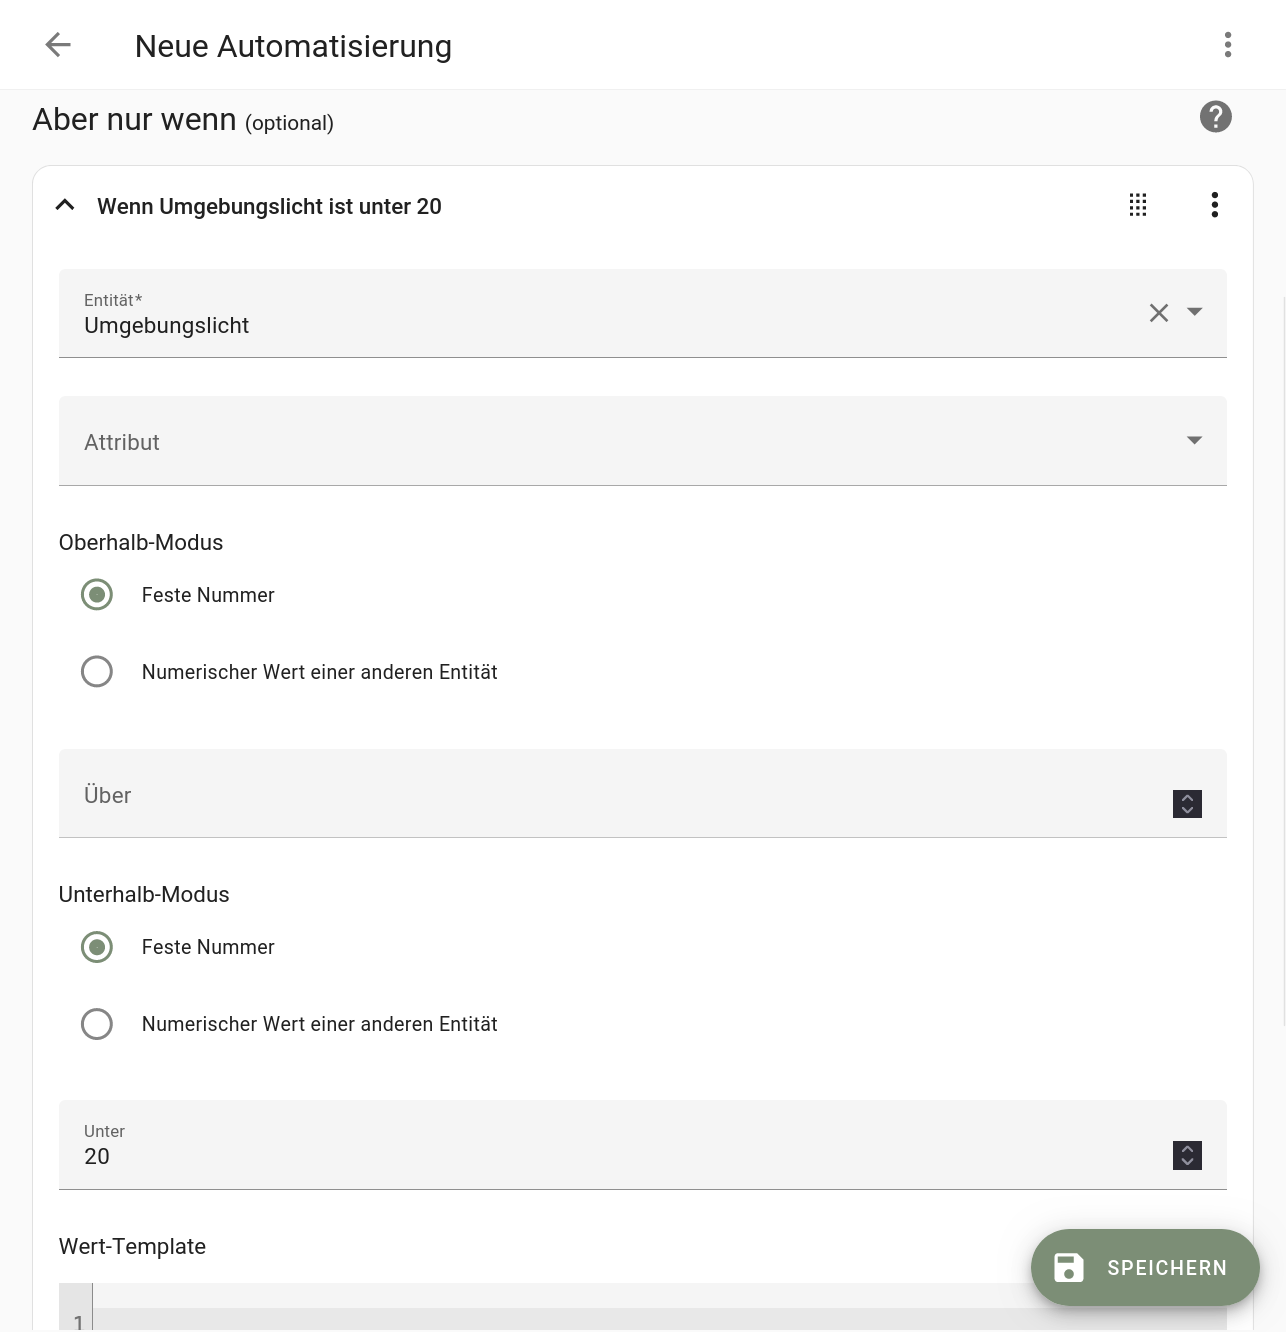
\includegraphics[width=\linewidth]{assets/hassio-automation-condition.png}
  \caption{Angabe einer Bedingung in Home Assistant}
  \label{figure:hassio-automation-condition}
  \endminipage
  \hfill
  \minipage[t]{.49\textwidth}
  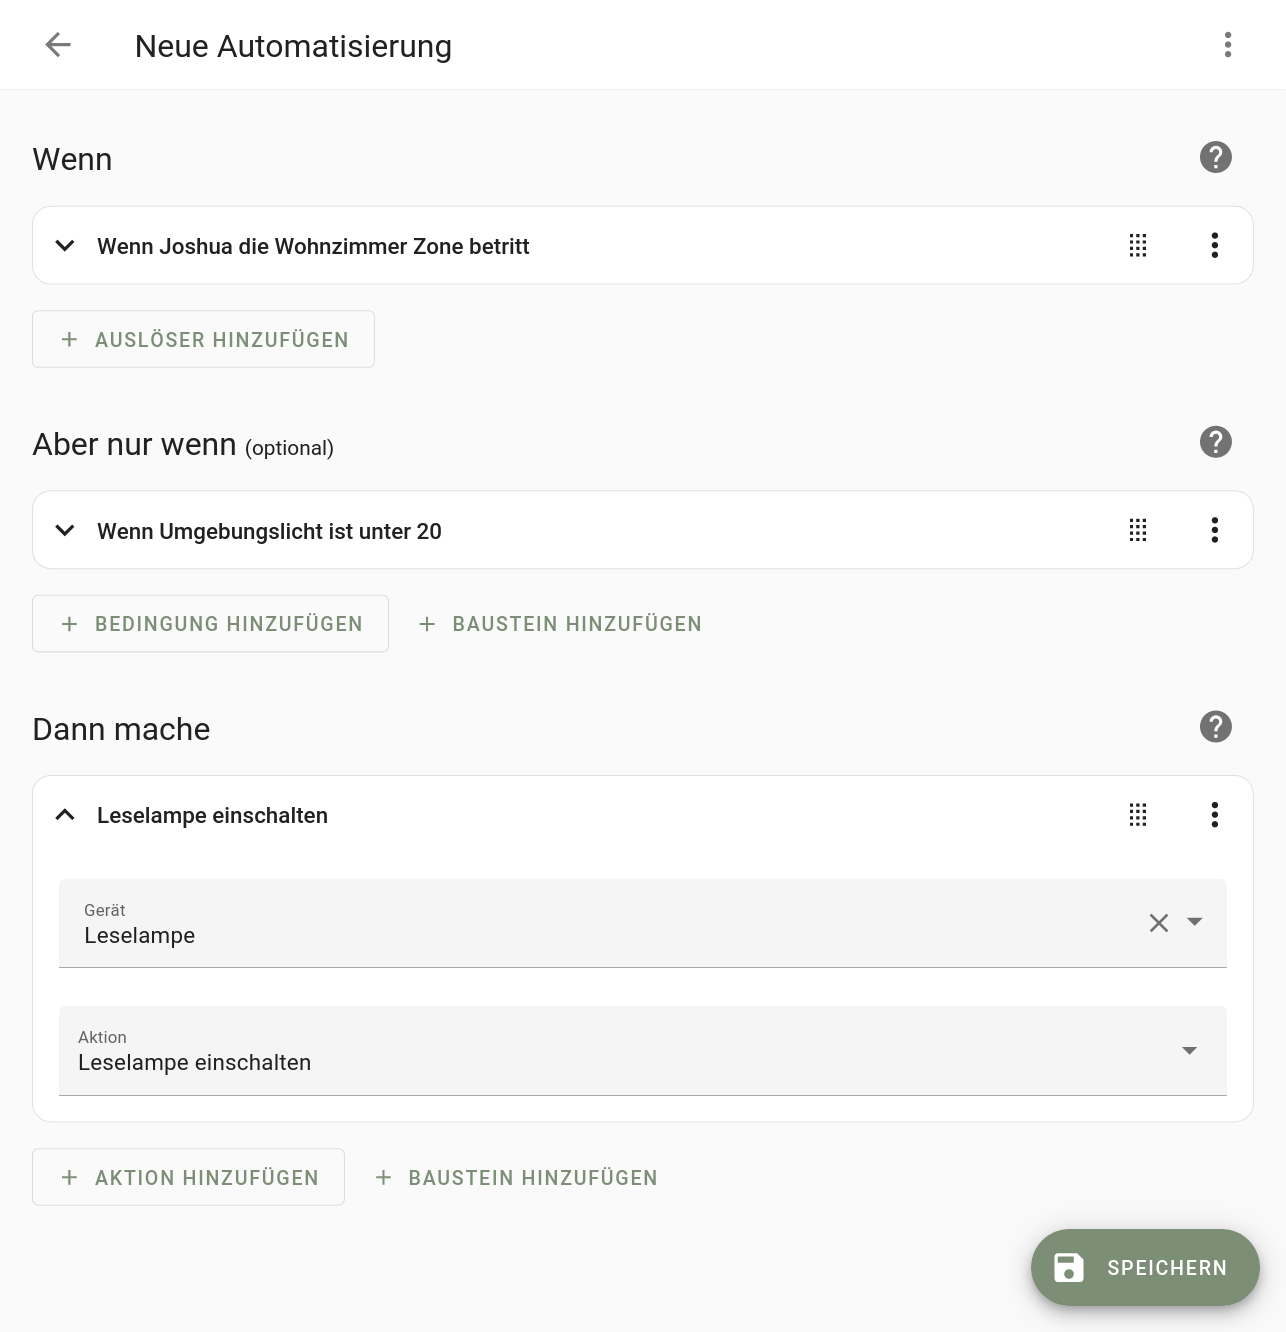
\includegraphics[width=\linewidth]{assets/hassio-automation-action.png}
  \caption{Angabe einer Aktion in Home Assistant}
  \label{figure:hassio-automation-action}
  \endminipage
\end{figure}
\todo{wegen Formattierung maybe 4 Abbildungen als eine figure definieren}

Abbildung \ref{figure:hassio-automation-action} zeigt den Endzustand beim Definieren einer
Automatisierung. Dazu wurde eine Aktion hinzugefügt, die die Entität "Leselampe" auf den Zustand
"An" setzt. Weitere Aktionen können über den Button "Aktion hinzufügen" hinzugefügt werden.
Komplexere Aktionsabläufe können über ein Pop-up-Fenster, welches Abbildung
\ref{figure:hassio-automation-trigger-select-1} und \ref{figure:hassio-automation-trigger-select-2}
ähnelt, ausgewählt werden. Beispielsweise können Aktionen gleichzeitig ausgeführt werden, oder
konditionale Strukturen gebildet werden \parencite{homeassistantScriptSyntax}.

\lstinputlisting[
  label=lst:automation,
  caption={\acs*{YAML}-Definition einer Automatisierung in Home Assistant},
  language=yaml,
  float=h,
]{assets/hassio-automation.yaml}

Die erstellte Automatisierung wird als Datei im \ac{YAML}-Format gespeichert. Quelltext
\ref{lst:automation} zeigt die aus der UI generierte \ac{YAML}-Datei. \todo{was noch mehr dazu?}
